\documentclass[11pt]{ctexart}
\usepackage[a4paper,margin=2.2cm]{geometry}
\usepackage{graphicx,booktabs,amsmath,amssymb,float,hyperref,xcolor,enumitem,fancyhdr,listings}
\hypersetup{colorlinks=true,linkcolor=blue,urlcolor=blue}
\setlist{itemsep=2pt,topsep=3pt,leftmargin=2em}
\setlength{\parskip}{3pt}
\setlength{\headheight}{14pt}
\lstset{basicstyle=\ttfamily\footnotesize,breaklines=true,breakatwhitespace=true,columns=fullflexible,frame=single,framerule=.2pt}
\pagestyle{fancy}\fancyhf{}\lhead{基于共享单车数据的交通需求预测}\rhead{课程分析报告}\cfoot{\thepage}
\newcommand{\fig}[3]{\begin{figure}[H]\centering\includegraphics[width=#2\linewidth]{#1}\caption{#3}\end{figure}}
\title{基于共享单车数据的交通需求预测\\\large 时空特征分析、短时建模与空间误差解释}
\author{}\date{}
\begin{document}\maketitle
\begin{abstract}
以深圳共享单车订单为基础，将城市划分为经纬网格并聚合为30分钟借还需求，使用过去24小时预测下一半小时30个区域的借还量。项目已实现历史平均、昨日同期、LSTM和Transformer。本文整理既有结果：主实验按70\%/15\%/15\%顺序划分，Transformer的MAE为61.01、RMSE为122.78、WMAPE为60.25\%，接近但未超过昨日同期基线。报告分析完整周日与周一的借还差异、高峰与平峰需求，以及网格间预测误差；另列日期划分实验，明确两套结果不能混用。由于样本时间覆盖严重不均衡，结论仅适用于当前样本。
\end{abstract}

\section{任务定义、数据与处理}
\subsection{预测目标与数据来源}
先分析共享单车需求的时空分布，再完成短时预测并与简单基线比较。预测对象是各区域未来30分钟的\textbf{借车量和还车量}。每到一个半小时预测点，使用此前已观测的24小时数据，滚动预测下一时段；测试时允许使用此前已经发生的真实需求，不是一次性预测后续多天。

项目实际使用深圳市政府数据开放平台“共享单车企业每日订单表”，API下载后保存到SQLite。原始库去重后有2,999,528条记录，混合2017年至2021年；本次研究使用2021年清洗订单，聚合脚本读取2,764,231条。字段为开始/结束时间及起点/终点坐标，用户标识不进入模型。现有材料没有证明该来源与课程统一发放文件完全一致，因此报告如实记录实际来源。

\subsection{清洗与时空聚合}
原始记录按哈希主键去重，清洗剔除缺失或无法解析的时间/坐标、结束时间不晚于开始时间、时长超过24小时、超出深圳近似边界、直线距离超过100 km、平均速度超过50 km/h等记录。

订单没有固定站点ID，故以$0.01^\circ\times0.01^\circ$网格代替站点，原点为纬度22.4、经度113.7。按全期借还总量选取30个高需求网格。订单开始时刻向下取整至半小时，在起点网格计一次借车；结束时刻同样取整，在终点网格计一次还车。补齐完整半小时索引得到$D\in\mathbb{R}^{1565\times60}$，列顺序为30个借车通道、30个还车通道。零槽表示样本没有记录，不保证真实需求为零；借还合计为事件数，不等于独立订单数。

\subsection{样本覆盖限制}
序列覆盖2021-01-01 00:00至2021-02-02 14:00。前29天在所选网格中的每日借还合计仅数百次，1月30日后大幅增加。图\ref{fig:daily}说明\textbf{采集样本时间覆盖不均}，不能据此判断真实城市需求突然增长数百倍。2月2日为不完整日，末端还车还受订单采样截断影响。
\begin{figure}[H]\centering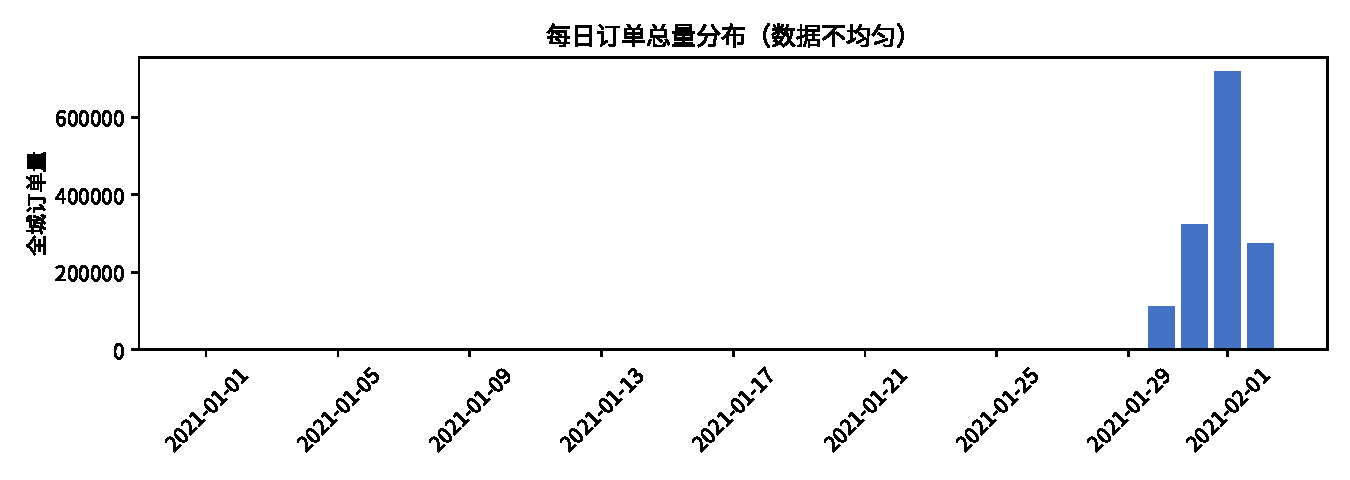
\includegraphics[width=.95\linewidth]{figs/daily_orders.pdf}
\caption{既有每日需求图。图内“全城订单量”应理解为所选30网格的借还事件合计，非全市完整订单量。}\label{fig:daily}\end{figure}

\section{需求时空特征}
\subsection{周末与工作日的借还差异}
高量段仅2021-01-31（周日）和2021-02-01（周一）是两个完整日，以下单独比较，不将不完整日混入日均值。工作日按周一至周五、周末按周六日标记，未引入法定节假日调休表。
\begin{table}[H]\centering\small\caption{完整日借还与日内结构：仅代表当前样本}
\begin{tabular}{lrr}\toprule
指标 & 01/31 周日 & 02/01 周一\\\midrule
全天借车事件/次 & 162,356 & 360,183\\
全天还车事件/次 & 161,451 & 358,761\\
早高峰借车占全天/\% & 12.75 & 24.90\\
晚高峰借车占全天/\% & 23.85 & 23.45\\
平峰借车占全天/\% & 56.19 & 44.33\\\bottomrule
\end{tabular}\end{table}
周一早间借车占比高于周日，周日白天更分散；周一全天借车约为周日2.22倍。但采集覆盖变化与日类型重叠，\textbf{不能将总量差异全部归因于工作日效应}，更不能用各一天归纳一般规律。

\subsection{早晚高峰、平峰与夜间}
与代码标记一致，早高峰为07:00--10:00，晚高峰为17:00--20:00，平峰为10:00--17:00及20:00--23:00，夜间为其余时段。不同类别时长不同，故采用\textbf{每半小时平均量}比较。每格为所选30网格合计的“借车/还车”。
\begin{table}[H]\centering\small\caption{时段借还强度（次/30分钟）}
\begin{tabular}{lrrr}\toprule
时段 & 每日槽数 & 周日（借/还） & 周一（借/还）\\\midrule
早高峰 & 6 & 3,449 / 3,653 & 14,945 / 16,114\\
晚高峰 & 6 & 6,453 / 6,492 & 14,078 / 13,380\\
平峰 & 20 & 4,562 / 4,477 & 7,984 / 7,836\\
夜间 & 16 & 732 / 691 & 1,648 / 1,568\\\bottomrule
\end{tabular}\end{table}
周一早晚高峰借车强度约为平峰1.87和1.76倍。早峰还车量高于借车量，晚峰借车高于还车，显示\textbf{所选区域集合}的净流入/流出差异，不能将其解释为全市车辆增减。周日早峰低于平峰，不能对所有日期概括相同双峰。
\fig{figs/high_volume_series.pdf}{.96}{既有高量段时序（30网格借还事件合计）。工作日早峰明显、周日白天较宽；末日中午骤降亦受采集终点影响。}

\subsection{空间单元与需求差异}
区域需求不均匀。网格ID定义为$1000g_y+g_x$，中心纬度$22.4+(g_y+0.5)\times0.01$、经度$113.7+(g_x+0.5)\times0.01$，可由元数据恢复地理位置。索引0对应网格14042，中心约为$(114.125^\circ E,22.545^\circ N)$。未融合POI，不能直接把网格命名为CBD、住宅区或地铁枢纽；空间误差分析见第5节。

\section{特征构造与预测模型}
\subsection{输入张量、时间编码和归一化}
对于待预测时刻$t$，使用$D_{t-48:t}$，即过去48步、24小时的60维借还需求。每个历史步另有\textbf{6维时间特征}：日内正弦/余弦、周内正弦/余弦、周末标记及高峰标记。设$m$为当日分钟数、$d$为星期索引，前四项为
\[\sin\frac{2\pi m}{1440},\quad\cos\frac{2\pi m}{1440},\quad
\sin\frac{2\pi(1440d+m)}{10080},\quad\cos\frac{2\pi(1440d+m)}{10080}.\]
再把目标的昨日同期$D_{t-48}$这60维复制至各历史步，故每步$60+6+60=126$维，实际\textbf{输入为$[B,48,126]$，输出为$[B,1,60]$}。不能把48个时间步展平后当成输入投影层的维度。

需求先做$\log(1+D)$，再以训练区间逐通道均值$\mu$和标准差$\sigma$做z-score；时间特征不做同一需求变换。验证、测试沿用训练统计量，测试数据不参与拟合归一化。

\subsection{残差学习与主实验配置}
记标准化对数需求为$z_t$，学习$r_t=z_t-z_{t-48}$，还原公式为
\[\hat D_t=\max\{\exp[(\hat r_t+z_{t-48})\sigma+\mu]-1,0\}.\]
残差位于\textbf{标准化对数域}，不是原始订单数直接相减。Transformer逐步投影126维输入，加位置编码，经时间编码器后取最后一步隐状态输出60维残差。各网格通道由多输出网络联合预测，没有显式的地理邻接图。
\begin{table}[H]\centering\small\caption{主实验既有检查点配置}
\begin{tabular}{lll}\toprule
配置 & Transformer & LSTM\\\midrule
输入/输出 & $48\times126$ / $1\times60$ & 同左\\
隐层/层数 & 32 / 1 & 64 / 1\\
注意力头/前馈层 & 4 / 64 & 不适用\\
dropout & 0.05 & 0\\
学习率/最大轮数 & $3\times10^{-5}$ / 100 & $10^{-4}$ / 80\\
优化/损失 & AdamW / Huber & AdamW / Huber\\
早停耐心/种子 & 20 / 42 & 15 / 42\\\bottomrule
\end{tabular}\end{table}
检查点分别为\texttt{transformer\_residual\_lr3e5}和\texttt{lstm\_residual}。可选“空间注意力”代码是隐通道的可学习混合，不等同于真实网格图上的图神经网络，故不作为已完成图建模成果。

\subsection{简单基线与公平比较}
历史平均按训练集“星期几$\times$半小时槽”求逐通道均值，未见槽回退至训练总体均值；昨日同期直接用$D_{t-48}$。LSTM使用相同输入、残差目标和时间划分。均在同一测试窗口、同一60通道上，还原原始计数后评估，不能用验证标准化损失代替订单数MAE。

\section{划分、指标与既有实验结果}
\subsection{主实验：70\%/15\%/15\%顺序划分}
1565步的训练终点索引1095、验证终点1330。前48步只作历史上下文；训练批次可随机打乱，但集合按目标时间顺序切分，不随机混分。
\begin{table}[H]\centering\small\caption{主实验目标窗口划分（时间均为半小时槽起点）}
\begin{tabular}{lllr}\toprule
集合 & 第一个目标 & 最后一个目标 & 窗口数\\\midrule
训练 & 01/02 00:00 & 01/23 19:00 & 1,047\\
验证 & 01/23 19:30 & 01/28 16:30 & 235\\
测试 & 01/28 17:00 & 02/02 14:00 & 235\\\bottomrule
\end{tabular}\end{table}
\textbf{限制：}训练和验证基本处于稀疏样本段，而测试包含高量段，存在严重分布偏移。滚动测试的昨日同期基线可使用此前已发生的测试期观测，这是合法单步在线设定，不能称为“抄答案”，也不等于固定起点多日预测。

\subsection{评价指标与主结果}
令$M$为测试槽$\times60$通道元素数，$e_i=\hat y_i-y_i$，使用
\[\mathrm{MAE}=\frac1M\sum_i|e_i|,\qquad\mathrm{RMSE}=\sqrt{\frac1M\sum_i e_i^2},\]
\[\mathrm{MAPE}_{\epsilon}=\frac{100}{M}\sum_i\frac{|e_i|}{\max(|y_i|,1)},\qquad
\mathrm{WMAPE}=100\frac{\sum_i|e_i|}{\max(\sum_i|y_i|,1)}.\]
MAE、RMSE单位为次/网格/30分钟（单个借或还通道）。RMSE更重视大误差。MAPE分母下限1处理零值，但低需求仍会放大相对误差，故结合MAE、RMSE和WMAPE解释。
\begin{table}[H]\centering\small\caption{主实验同一测试集结果（来自既有指标文件）}
\begin{tabular}{lrrrr}\toprule
模型 & MAE & RMSE & MAPE$_\epsilon$(\%) & WMAPE(\%)\\\midrule
历史平均 & 101.20 & 198.86 & 72.29 & 99.93\\
昨日同期 & \textbf{60.41} & \textbf{122.22} & 584.94 & \textbf{59.65}\\
LSTM残差 & 62.34 & 124.29 & 518.29 & 61.55\\
Transformer残差 & 61.01 & 122.78 & 564.90 & 60.25\\\bottomrule
\end{tabular}\end{table}
\fig{figs/model_compare.pdf}{.85}{既有主实验MAE/RMSE图，属于比例划分，与下节日期实验不同。}
Transformer相对历史平均MAE下降约39.71\%，却比昨日同期高约1.00\%；LSTM也未超过昨日同期，\textbf{不能声称复杂模型优于全部基线}。历史均值的MAPE较低而MAE更大，反映低量槽对MAPE排名的影响。

\subsection{补充：高量段日期划分实验}
另一套既有实验的训练目标为01/30 13:00--01/31 19:30（62窗），验证01/31 20:00--02/01 03:30（16窗），测试02/01 04:00--02/02 14:00（69窗）。首批训练输入仍使用起点前24小时历史，不能称历史输入全部高量。其Transformer为64隐层、2层、4头、前馈128、dropout 0.05、学习率$10^{-4}$，检查点\texttt{transformer\_date\_full}。
\begin{table}[H]\centering\small\caption{补充日期实验：不同测试集，不能直接与主实验相减}
\begin{tabular}{lrrr}\toprule
模型 & MAE & RMSE & WMAPE(\%)\\\midrule
历史平均（原实现） & 231.73 & 339.44 & 98.44\\
昨日同期 & 124.36 & 203.91 & 52.83\\
Transformer残差 & 133.23 & 216.48 & 56.60\\\bottomrule
\end{tabular}\end{table}
该历史平均的回退均值从序列起点取至训练终点，包含早期稀疏样本，不是仅用62个高量时点；这里保留原实现结果。没有既有同日期划分的LSTM结果，故不填空或借用比例实验。该实验亦未证明Transformer超越昨日同期。

\section{空间误差与原因分析}
\subsection{网格误差分布与地理对应}
主实验的网格借/还MAE分别在235个目标上平均。图按元数据需求排名索引0--29显示误差，是\textbf{空间单元间比较}，不能误称为带底图的地理热力图。
\fig{figs/spatial_error.pdf}{.98}{主实验Transformer的30网格借/还MAE。编号为数组索引，非行政区或站点名。}
\begin{table}[H]\centering\small\caption{高误差网格的空间对应（BD09原始坐标）}
\begin{tabular}{rrrrr}\toprule
图中索引 & 网格ID & 中心经度 & 中心纬度 & 借还平均MAE\\\midrule
0 & 14042 & 114.125 & 22.545 & 113.98\\
1 & 14041 & 114.115 & 22.545 & 94.92\\
2 & 14038 & 114.085 & 22.545 & 89.34\\
5 & 13035 & 114.055 & 22.535 & 74.34\\
3 & 12034 & 114.045 & 22.525 & 72.35\\\bottomrule
\end{tabular}\end{table}
借车总体MAE约61.47，还车约60.56。网格0的借还平均MAE约113.98，显著高于不少后部网格的约45--60。30网格平均真实需求与其平均MAE的Pearson相关系数约0.98，支持\textbf{本样本中高需求规模与高绝对误差相关}；不证明相对误差或土地利用因果。

\subsection{时间分组与误差解释}
\begin{table}[H]\centering\small\caption{主实验Transformer的分时段误差}
\begin{tabular}{lrrr}\toprule
时段 & 测试槽数 & MAE & WMAPE(\%)\\\midrule
早高峰 & 30 & 116.26 & 49.14\\
晚高峰 & 30 & 93.60 & 58.98\\
平峰 & 95 & 73.86 & 70.14\\
夜间 & 80 & 12.82 & 52.94\\\bottomrule
\end{tabular}\end{table}
分组包含稀疏与高量日期，不代表独立多周评估。早峰MAE最高、夜间最低，空间误差可作如下解释：
\begin{enumerate}
\item \textbf{规模效应：}大流量区域即使同比例误差，也会对应更大绝对偏差；网格图与相关系数支持这一样本描述。
\item \textbf{日型转换与样本不足：}高量段仅几天，周日到周一早峰结构变化，训练数据不足以学习稳定的残差修正。
\item \textbf{采集偏移与选择：}低量训练、高量测试及末日不完整会影响偏差；30网格按全期热度选择，包含测试期空间筛选信息。只用训练集归一化不等于完全排除了选择偏差。
\item \textbf{未验证解释：}天气、活动、轨道接驳和POI可能影响局部需求，但未融合相应数据，不能写作已经证实的成因。
\end{enumerate}

\section{结论、局限与可运行代码}
已完成订单清洗、半小时借还聚合、日类型与高峰样本分析、基线和神经模型比较，以及空间误差分解。主实验Transformer MAE为61.01，昨日同期60.41；日期实验分别133.23和124.36，两者都未证明Transformer优于昨日同期。

后续优先补充覆盖一致的连续多周数据、仅用训练期选区域，采用多个滚动起点测试；再加入上一时段持久性基线、天气、POI或真实空间结构。上述是\textbf{后续建议}，不列为已完成实验。周末/工作日各只有一个完整高量日，时间覆盖偏移、单切分和小样本限制了泛化结论。

代码随项目提交，依赖见\texttt{requirements.txt}。聚合、Transformer与LSTM的入口分别为：
\begin{itemize}\small
\item \path{src/aggregate_demand.py}
\item \path{src/train_transformer.py}
\item \path{src/train_lstm.py}
\end{itemize}
检查点目录（各含指标与预测文件）：
\begin{itemize}\small
\item 主实验Transformer：\path{checkpoints/transformer_residual_lr3e5}
\item 主实验LSTM：\path{checkpoints/lstm_residual}
\item 日期实验：\path{checkpoints/transformer_date_full}
\end{itemize}
通用说明见\path{docs/training_pipeline.md}，本实验参数以下方命令为准。部分旧预测文件的\texttt{times}字段单位异常，主实验日期按聚合数组的测试索引核对。项目原有仓库地址为\url{https://github.com/wyyy520/BikeDemand}。

以下命令可从项目根目录运行；依赖安装步骤按项目环境选择执行。
\begin{lstlisting}
python -m pip install -r requirements.txt
python src/aggregate_demand.py --input data/processed/orders_2021_clean.sqlite --output data/processed/demand_2021_30min.npz --top-grids 30
python src/train_transformer.py --data data/processed/demand_2021_30min.npz --output-dir checkpoints/reproduce_transformer --d-model 32 --nhead 4 --layers 1 --ffn-dim 64 --dropout 0.05 --lr 0.00003 --epochs 100 --patience 20
python src/train_lstm.py --data data/processed/demand_2021_30min.npz --output-dir checkpoints/reproduce_lstm --hidden-dim 64 --layers 1 --dropout 0 --lr 0.0001 --epochs 80 --patience 15
\end{lstlisting}
默认lookback为48、horizon为1、种子42、批量64，比例划分70\%/15\%。

\appendix\section{既有过程素材与小组协作}
\fig{爬取300万数据集数据库.png}{.66}{原有数据采集截图，仅作为实现过程证据，不代替分析图。}
\begin{figure}[H]\centering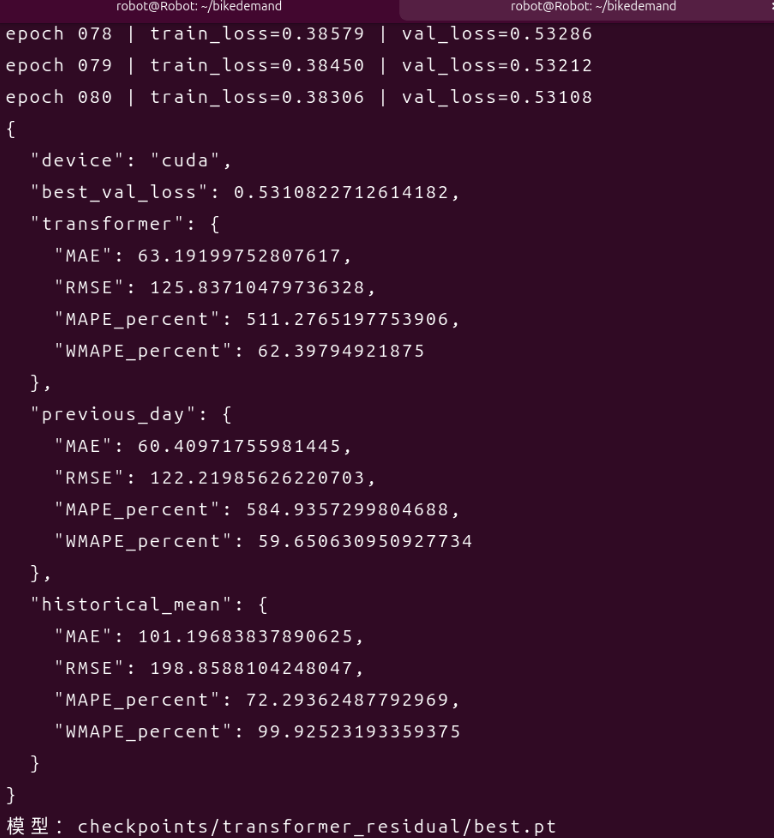
\includegraphics[width=.46\linewidth]{优化后的transformer.png}\hfill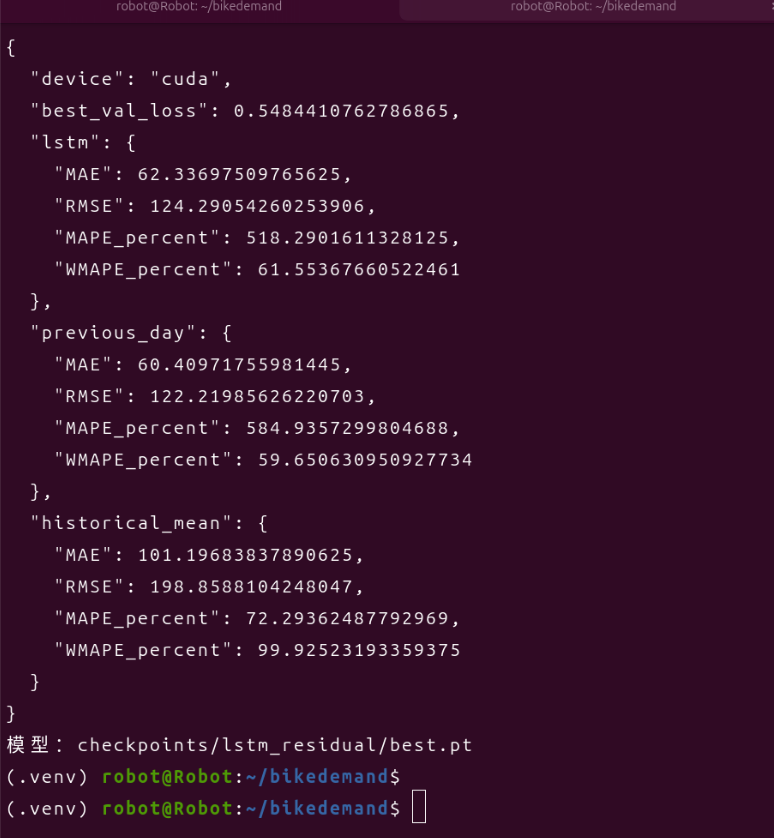
\includegraphics[width=.46\linewidth]{优化后的lstm.png}\caption{原有调试过程截图，可能对应不同版本，不代替已标明检查点的正式指标表。}\end{figure}
课程要求4--6人共同讨论与分工。尚未提供真实姓名、学号及具体贡献，以下留待小组填写，实际共同制定的方案与分工应据实补充。
\begin{table}[H]\centering\small\begin{tabular}{p{.25\linewidth}p{.62\linewidth}}\toprule
姓名/学号 & 实际承担工作与共同讨论内容\\\midrule
\rule{0pt}{2.8ex} & \\
\rule{0pt}{2.8ex} & \\
\rule{0pt}{2.8ex} & \\
\rule{0pt}{2.8ex} & \\
\rule{0pt}{2.8ex} & \\
\rule{0pt}{2.8ex} & \\\bottomrule\end{tabular}\end{table}
\end{document}
